\begin{frame}
\centering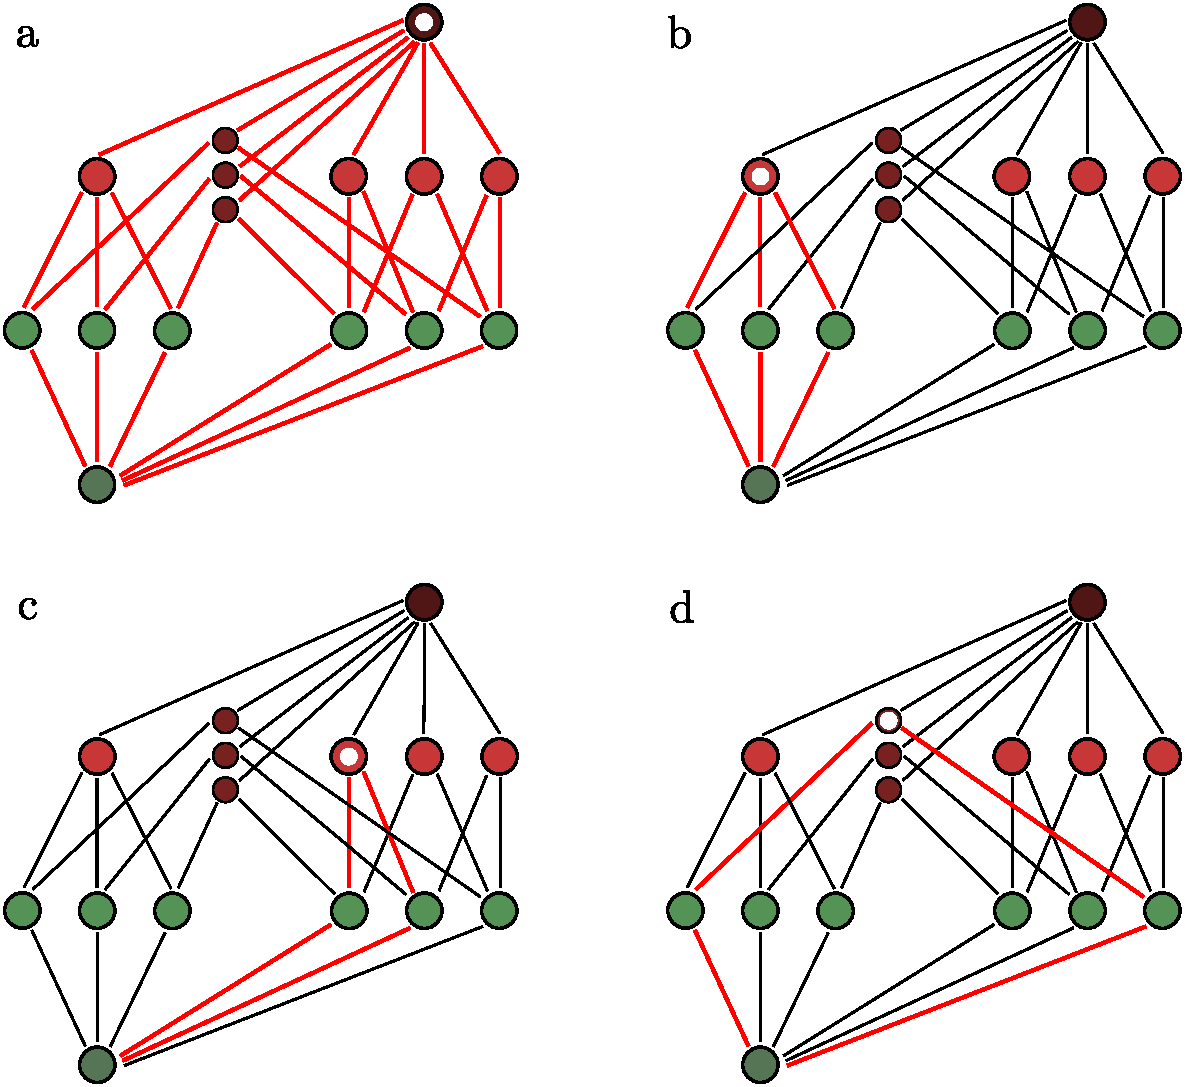
\includegraphics[width=0.4\textwidth]{fig/sieveHasseNoNum.pdf}
\begin{block}{sieves conceptualized on {\it Hasse diagrams} of an algebraic lattice}
All edges are directed from bottom to top. Red edges are part of a sieve on an object represented by a node in the lattice. Black edges are part of the lattice but not part of the sieve under consideration. (a) shows the maximal sieve on the lattice, which is equivalent to a sieve on the object marked with a white dot. (b), (c), and (d) show maximal sieves on the respective objects marked with white dots.
\end{block}
\end{frame}